\documentclass[10pt, twocolumn, a4paper]{article}

% --- Packages ---
\usepackage[utf8]{inputenc}
\usepackage[T1]{fontenc}
\usepackage{geometry}
\usepackage{titlesec}
\usepackage{titling}
\usepackage{amsmath, amssymb}
\usepackage{graphicx}
\usepackage{booktabs}
\usepackage{enumitem}
\usepackage{multicol}
\usepackage{xcolor}
\usepackage{caption}
\usepackage{eso-pic}
\usepackage{hyperref}
\usepackage{float}

% --- Standard Academic Layout (Relaxed for Multi-Page) ---
\geometry{top=2.0cm, bottom=2.0cm, left=1.5cm, right=1.5cm, columnsep=0.6cm}
\setlength{\parindent}{0pt}
\setlength{\parskip}{4pt}
\setlist[itemize]{leftmargin=*, nosep, topsep=3pt, itemsep=2pt}
\setlist[enumerate]{leftmargin=*, nosep, topsep=3pt, itemsep=2pt}
\setlist[description]{leftmargin=*, nosep, topsep=3pt, itemsep=2pt}
\titlespacing*{\section}{0pt}{8pt}{4pt}
\titlespacing*{\subsection}{0pt}{4pt}{2pt}

% --- Hyperlink Setup ---
\hypersetup{colorlinks=true, linkcolor=blue, urlcolor=cyan}

\begin{document}

% --- Logo Placement ---
\AddToShipoutPictureBG*{
  \AtPageUpperLeft{
    \hspace{1.5cm}\raisebox{-1.5cm}{
      % Ensure your logo is in the same folder
      
\includegraphics[height=1.5cm]{images/logo.png}
    }
  }
}

% --- Custom Header Block ---
\twocolumn[{
  \begin{center}
    {\LARGE \textbf{Camera-Based Real-Time Exercise Classification and Technique Feedback for Telerehabilitation}\par}\vspace{2ex}
    {\normalsize \textbf{Ahmed Loay}\textsuperscript{1}, \textbf{Mo'men Mohamed}\textsuperscript{2}, \textbf{Rawan Mohamed}\textsuperscript{3}, \textbf{Youssef Mohamed}\textsuperscript{4} \\ \textit{\textsuperscript{1}Cairo University, Faculty of Engineering}}\\[2ex]
  \end{center}
  
  \noindent\textbf{\normalsize Abstract---}\small This project develops a real-time, vision-based system that classifies rehabilitation exercises from a single camera and provides instantaneous feedback on movement technique. By replacing subjective observation with objective, automated analysis, the system enables patients to perform exercises correctly at home, reduces the need for in-person visits, and helps prevent secondary injuries caused by improper form.
  
  \vspace{8mm} % Generous space before the two columns begin
}]

% --- Line Spacing ---
\renewcommand{\baselinestretch}{1.15}\normalsize

\section{Significance of the Problem}
Traditional physical rehabilitation relies on periodic, in-person evaluations by a physiotherapist, which limits accessibility and can delay correction of improper technique. Automating this process using a standard smartphone camera \textbf{democratizes access} to high-quality care and enables continuous monitoring. Key benefits:
\begin{itemize}
    \item \textbf{Real-Time Feedback:} Instant audio/visual cues guide patients to correct posture during exercise, preventing ingrained mistakes.
    \item \textbf{Objective Quantification:} Converts qualitative observations into precise joint angles and movement metrics, allowing accurate progress tracking.
    \item \textbf{Scalable Telerehabilitation:} Supports remote therapy programs, reducing healthcare costs and improving adherence.
\end{itemize}

\section{Market Analysis}
The digital musculoskeletal (MSK) rehabilitation market is expanding rapidly, yet existing commercial solutions generally fall into paradigms that compromise either accessibility, computational efficiency, or clinical explainability.

\begin{itemize}
    \item \textbf{Hardware-Dependent Systems:} Market leaders like Hinge Health (\$6.2B valuation) and Sword Health (\$2B valuation) rely on proprietary wearable inertial sensors. Similarly, legacy systems like Reflexion Health utilized depth cameras. While highly accurate, these approaches introduce friction, requiring logistical hardware distribution and increasing per-patient costs.
    \item \textbf{Deep Learning Vision Systems:} Companies like Kaia Health and Kemtai utilize smartphone cameras powered by heavy deep learning models (e.g., BlazePose variants). While solving the hardware accessibility problem, these "black-box" models lack clinical transparency. When a model fails, it is difficult for a clinician to understand \textit{why}, and running these models natively on older smartphones severely drains battery and compute resources.
    \item \textbf{Passive Video Platforms:} Solutions like PhysiApp provide digital home exercise programs but lack automated movement analysis, relying entirely on patient self-reporting.
\end{itemize}

\textbf{Unique Value Proposition:} The proposed system bridges a critical gap in the market. By utilizing classical machine learning (SVMs, Pictorial Structures, HOG) on standard smartphone RGB streams, the system achieves the hardware accessibility of Kaia and Kemtai while offering the deterministic explainability and ultra-low computational footprint required for mass deployment in diverse socio-economic settings.


\section{Literature Review}
The proposed pipeline is grounded in canonical computer vision literature, specifically leveraging classical techniques that provide clinical explainability and computational efficiency.

\textbf{Pose Estimation Framework:} The core of our spatial modeling relies on the Pictorial Structures (PS) framework, originally introduced by Fischler and Elschlager \cite{fischler1973representation}, which models the human body as a collection of rigid templates connected by deformable springs. Felzenszwalb and Huttenlocher \cite{felzenszwalb2005pictorial} demonstrated that dynamic programming inference on these tree-structured models operates in linear time, rendering the approach computationally tractable for real-time applications. Subsequent extensions by Yang and Ramanan \cite{yang2011articulated} handling flexible mixtures of parts inform our strategy for managing viewpoint variability.

\textbf{Feature Extraction \& Segmentation:} To isolate the kinematic signal without relying on dense neural networks, we utilize Histogram of Oriented Gradients (HOG), established by Dalal and Triggs \cite{dalal2005histograms} as the premier descriptor for human detection. For environment isolation, our background subtraction module builds upon the foundational Gaussian Mixture Model (GMM) work by Stauffer and Grimson \cite{stauffer1999adaptive}, enhanced by Zivkovic's \cite{zivkovic2004improved} adaptive Gaussian selection and Horprasert et al.'s \cite{horprasert1999statistical} shadow suppression techniques.

\textbf{Temporal Modeling \& Evaluation:} Because classical 2D pose estimation suffers from high-frequency jitter, we implement Extended Kalman Filtering (EKF), adapting the articulated tracking principles established by Sminchisescu and Triggs \cite{sminchisescu2004kinematic}. For system evaluation, we adopt the Mean Per Joint Position Error (MPJPE) metric standardized by Sigal et al. \cite{sigal2010humaneva} in the HumanEva benchmark. 

\textbf{Clinical Context \& Baselines:} Choi et al. \cite{choi2017exergame} established the clinical necessity for automated movement assessment. Historically, systems like the Microsoft Kinect \cite{shotton2011real} dominated this space. Work by Kurillo et al. \cite{kurillo2013kinect} evaluating Kinect-based workspaces provides the performance baseline ($\approx$15mm joint accuracy) that our single RGB camera system aims to approach. Furthermore, while standard datasets like Leeds Sports Pose (LSP) provide athletic poses, a notable gap remains in datasets featuring controlled, clinical rehabilitation movements, necessitating targeted fine-tuning for this domain.


\section{Challenges \& Mitigation}
Like any system that tries to do something meaningful in the real world, ours ran into friction fast. Patients don't exercise in controlled lab environments — they move in cluttered living rooms, on shaky phone mounts, under inconsistent lighting. Early in development, it became clear that the classical computer vision toolkit, while theoretically sound, was brittle the moment conditions deviated. So we made a deliberate architectural decision: ditch fragile background subtraction and heavyweight deep models entirely, and instead build a leaner, two-stage kinematic pipeline that could actually survive real-world conditions. Three challenges shaped that decision most.

\begin{enumerate}[label=\textbf{\arabic*.}]
    \item \textbf{Environments Don't Cooperate:} Gaussian Mixture Models (GMM) are elegant on paper, but in practice they fall apart the moment a fan turns on, a curtain moves, or someone walks through the background. The model doesn't know what to do with that — it wasn't designed to. Rather than patch a fundamentally fragile approach, we switched to MediaPipe's topological landmark extraction, which tracks the person directly, not the background. The subject stays detectable regardless of what's happening around them.

    \item \textbf{Real-Time Is a Hard Constraint, Not a Nice-to-Have:} A feedback system that lags is worse than no feedback at all — it confuses patients about what they're doing wrong. The naive implementation of running full ML inference on every single frame bottlenec the UI thread down to unworkable framerates. So, we decoupled inference entirely from rendering. A background worker handles the heavy computation on its own schedule, while the UI thread runs clean at 30+ FPS. The user always sees a smooth experience, and the models always get clean, unhurried computation.

    \item \textbf{There Is No Ground Truth:} This was the most uncomfortable reality of the project. No major dataset ships with frame-by-frame clinical quality annotations. A physiotherapist doesn't label every squat in a video file. We couldn't simply supervise our quality model the conventional way. Our answer was a \textbf{self-supervised} proxy labeling system: during training, an Isolation Forest scores each repetition against the population distribution, mathematically flagging deviations from the statistical norm. It's not a clinician's judgment, but it's rigorous, reproducible, and far better than guessing.
\end{enumerate}

\section{Proposed System Overview}
At its core, the system is a software-defined diagnostic tool that runs entirely through a single RGB camera — no wearables, no depth sensors, nothing that needs to be shipped or charged. A patient just opens the application, stands in front of their phone or laptop camera, and starts moving.

The pipeline takes a continuous live video stream as input and produces two things simultaneously: a prediction of which exercise the user is performing, and a continuous quality score between 0 and 1 that reflects how well they're executing it. Both are displayed in real time on a clinical heads-up display, overlaid on the live skeletal tracking visualization so patients can immediately see what needs correcting. The full implementation is publicly available: \href{https://github.com/rawan-mohamed-n/Action_Prediction_Using-_Penn_Action}{Action Prediction \& Evaluator}.

\begin{figure}[H]
    \centering
    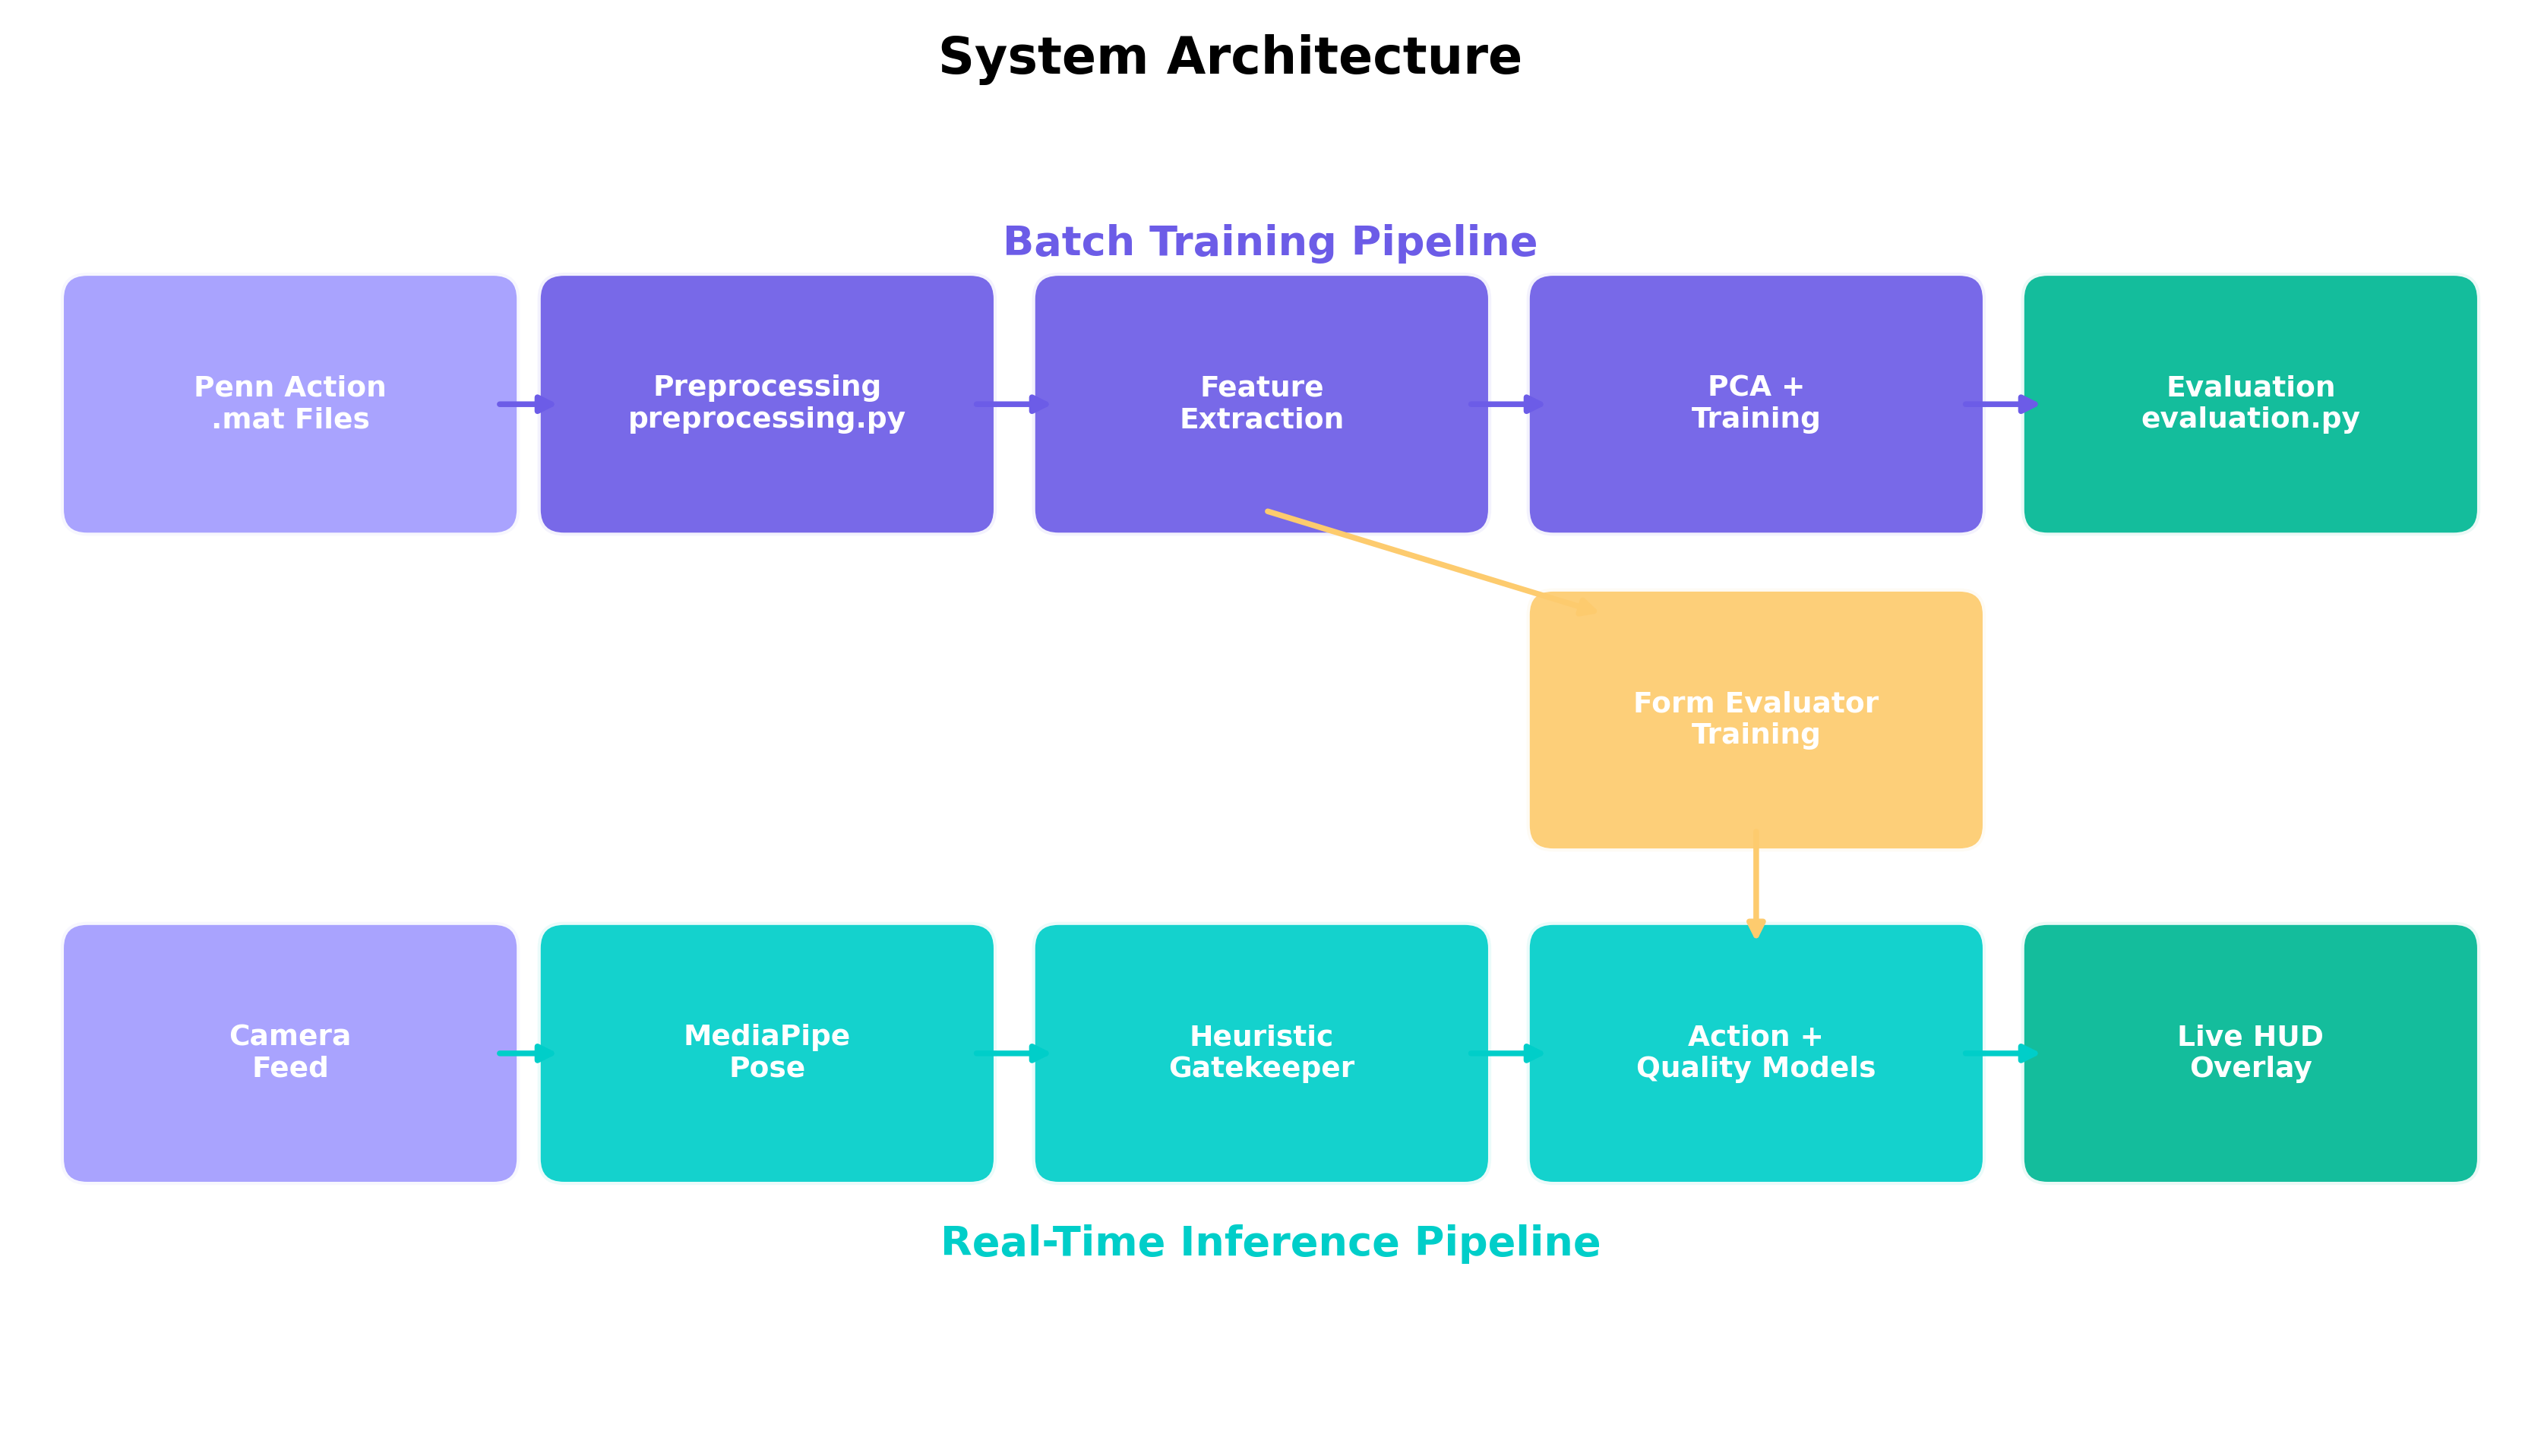
\includegraphics[width=\columnwidth]{figures/fig1_architecture.png}
    \caption{System Architecture Diagram detailing the data flow from raw RGB frames through MediaPipe spatial extraction, gatekeeping, decoupled asynchronous buffers, and the dual-stage classification and quality scoring modules.}
    \label{fig:architecture}
\end{figure}

\section{Machine Learning Pipeline}

\subsection{Module 1: Spatial Extraction \& Gatekeeping}
Every frame that comes off the camera gets processed first by MediaPipe Pose, which extracts 33 three-dimensional body landmarks in real time. This replaces background subtraction entirely — rather than trying to figure out what isn't the person, we go straight to modeling what is.

But raw landmark data has a problem: when a patient stops moving, or when the camera fails to detect them cleanly, there's no useful signal. Feeding that empty noise into a classifier produces confident, completely wrong predictions — what the field sometimes calls ``hallucinated'' outputs. To prevent this, every frame passes through a \textbf{Heuristic Gatekeeper} before it ever reaches the ML models:

\begin{itemize}
    \item \textbf{Visibility Check:} If a frame doesn't contain a full set of detectable landmarks, it gets dropped immediately. No landmarks, no inference — it's that simple.
    \item \textbf{Idle State Detection:} Even when landmarks are present, the system checks whether the person is actually moving. It computes the variance of core Y-coordinates (hips and shoulders) across a rolling 5-frame window. When that variance drops below a threshold of $0.001$, the subject is flagged as ``Idle,'' and the inference pipeline pauses. This isn't just a computational optimization — it also protects the quality scoring model from being diluted by stationary data that carries no kinematic information.
\end{itemize}

\subsection{Module 2: Decoupled Asynchronous Buffers}
A single frame is a photograph — it tells you where the joints are, but nothing about how they're moving. Meaningful kinematic analysis requires history: range of motion, velocity, symmetry, and repetition structure only emerge across time. The system handles this by maintaining two distinct memory buffers running in parallel, each tuned to a different analytical need:

\begin{itemize}
    \item \textbf{Fast Action Buffer (30 Frames):} A tight, one-second rolling window designed for responsiveness. This buffer feeds the action classifier, giving it enough trajectory context to identify what exercise is being performed without waiting for an entire repetition to complete.
    \item \textbf{Deep Quality Buffer (90 Frames):} A wider, three-second window that captures the full arc of a slow, controlled movement. This is what the quality scorer reads from — it needs the complete picture of a repetition to reliably compute maximum joint angles, minimum positions, and coordinate spread.
\end{itemize}

One subtle but critical implementation detail: landmarks extracted by MediaPipe are normalized to the frame dimensions. Before features are computed, these coordinates are re-scaled back to absolute pixel space to ensure mathematical consistency with the training distribution the models were built on.

\subsection{Module 3: Stage 1 --- Action Classification}
The first stage answers a deceptively simple question: \textit{what exercise is this person doing?} The Fast Action Buffer is summarized into 62 statistical features — the minimum, maximum, average, variance, and standard deviation of each landmark coordinate across the window. This compact vector is passed to a \textbf{Random Forest Classifier}, which maps it to one of the supported exercise categories: Squat, Pushup, Jump Rope, and others.

The design intent here matters. By automating exercise identification, the system removes the need for patients to select their current activity manually. They can move fluidly through a session, and the classifier follows them seamlessly — an important quality-of-life detail for patients who may be elderly, recovering from injury, or simply unfamiliar with technology.

\subsection{Module 4: Stage 2 --- Kinematic Quality Scoring}
The second stage is where the system earns its clinical value: it doesn't just know \textit{what} you're doing, it tells you \textit{how well} you're doing it. Since no dataset provides therapist-annotated quality labels, the system generates its own ground truth during training using self-supervision.

An \textbf{Isolation Forest} — an anomaly detection algorithm — processes every training repetition and assigns an outlier score relative to the population average. Repetitions that deviate significantly from the statistical norm score low; those that closely match the distribution score high. These scores are normalized into a continuous $[0, 1]$ quality baseline.

During live inference, the 90-frame Deep Quality Buffer is summarized into the same statistical feature space, enriched with the one-hot encoded exercise label from Stage 1. This combined vector is fed into a \textbf{Random Forest Regressor}, which outputs the final quality score. The result is a number the patient can actually act on — not a vague warning, but an objective, quantitative measure of how their current form compares to what a correct repetition looks like.

\section{Dataset \& Strategy}
The models were trained on the \textbf{Penn Action Dataset}, a collection of diverse, unconstrained athletic video sequences captured in real-world settings with moving cameras and unpredictable backgrounds. The choice was deliberate. A system trained only on clean, studio-recorded footage would have no idea what to do in a patient's actual home environment.

By training on Penn Action's messy, dynamic footage, the pipeline was forced to learn kinematic patterns from statistical features rather than visual appearance cues — which is exactly the right lesson. Joint angle distributions, velocity profiles, and coordinate variance are properties of human movement. Background clutter is not. That distinction is what allows the system to generalize, and it's what separates a genuinely deployable tool from a research demo that only works under controlled conditions.

\subsection{Penn Action Data Structure}
Each of the 2,326 Penn Action sequences ships as a MATLAB \texttt{.mat} file containing three parallel arrays: a $T \times 13$ matrix of X-coordinates, a matching matrix of Y-coordinates, and a binary $T \times 13$ visibility mask — where $T$ is the number of frames and 13 is the number of tracked anatomical keypoints. The skeleton model covers Head, bilateral Shoulders, Elbows, Wrists, Hips, Knees, and Ankles, connected into a kinematic tree of 12 limb segments. Metadata fields provide the action label, frame count, and viewpoint.

The important subtlety here is the visibility mask. When a joint is occluded — a wrist hidden behind the torso during a pushup, an ankle disappearing below the frame edge — the dataset still provides coordinate values, but they are unreliable. A naive pipeline that trusts those coordinates blindly produces geometry that doesn't correspond to the actual human body. Our preprocessing addresses this head-on.

\begin{figure}[H]
    \centering
    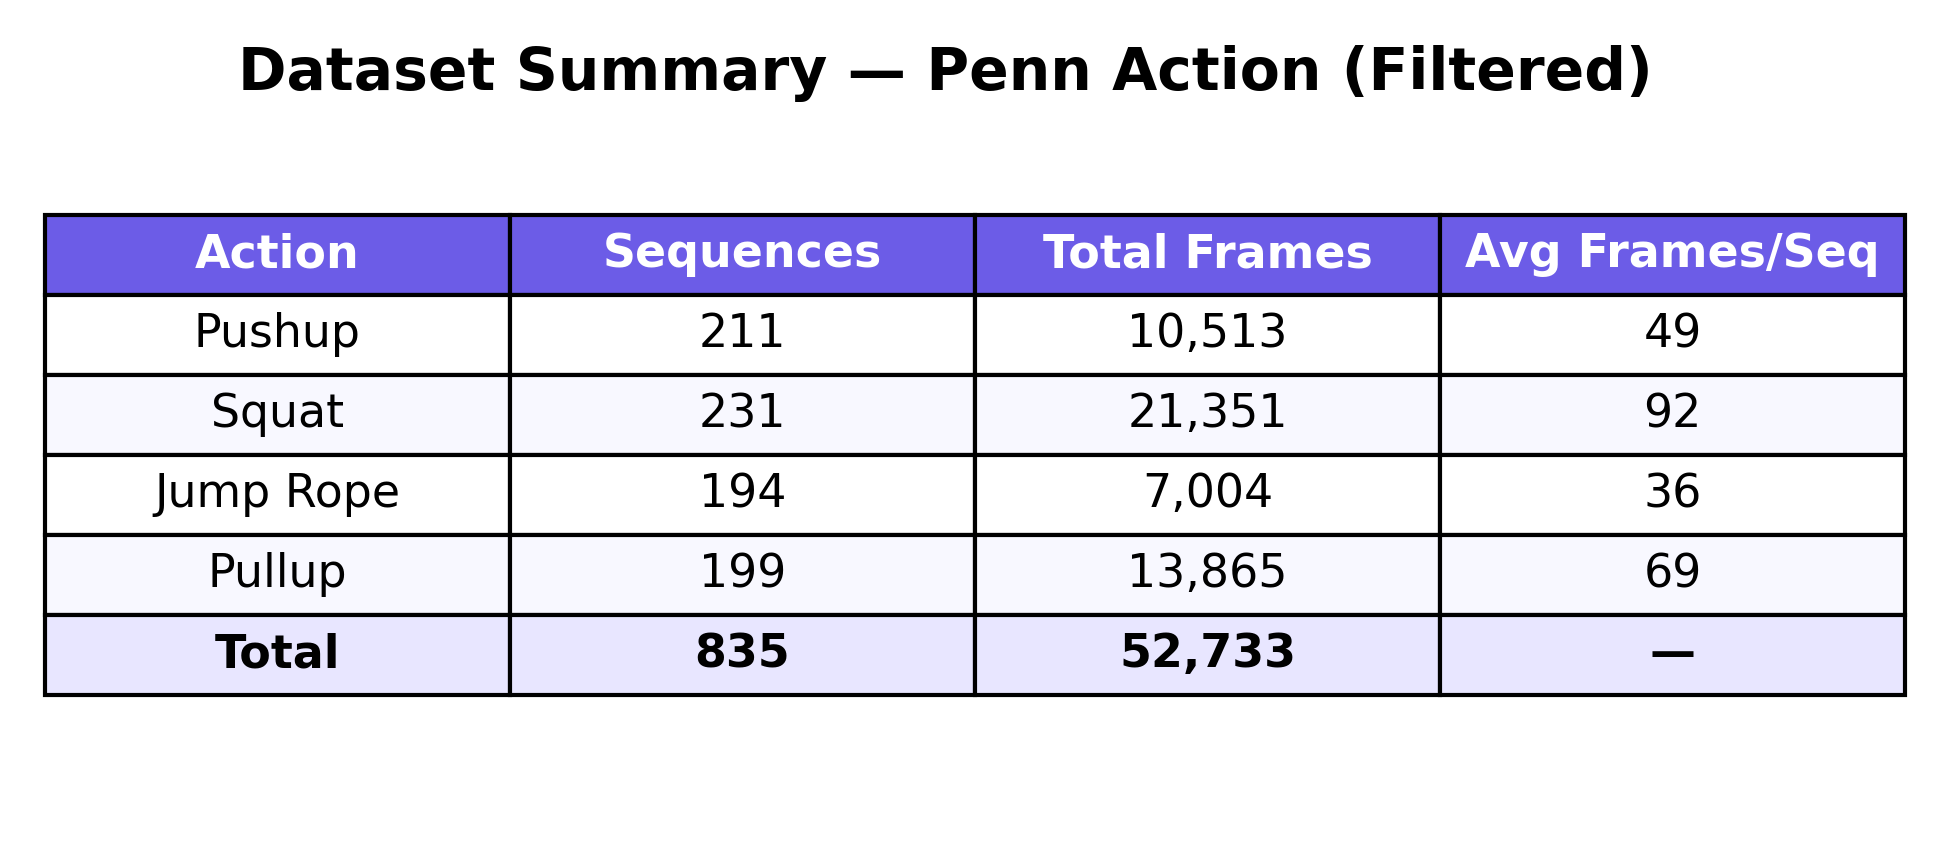
\includegraphics[width=\columnwidth]{figures/fig2_dataset_stats.png}
    \caption{Dataset statistics detailing the distribution of sequences across target exercises. Class imbalances were mitigated by using balanced class weighting during training.}
    \label{fig:dataset_stats}
\end{figure}

\subsection{Preprocessing: From Raw Annotations to Clean Kinematics}
The raw data presents three distinct problems that need to be solved before anything useful can be extracted: occluded joints carry corrupted coordinates, missing joints leave gaps in the temporal signal, and camera viewpoint introduces systematic geometric distortion. We handle each in sequence.

\subsubsection{Visibility-Aware Loading}
The first step is honest: we don't pretend to know where an invisible joint is. Every joint with $\texttt{visibility} = 0$ is explicitly replaced with \texttt{NaN}. This is a deliberate design choice — it's better to have a missing value that downstream methods can reason about than a confident but wrong number that silently corrupts every distance and angle computed from it.

\subsubsection{Mirror Symmetry Correction}
In front-facing sequences, the human body is approximately bilaterally symmetric. When one side's joint is visible but its contralateral counterpart is missing, we exploit that symmetry to estimate the occluded position. The missing joint is reflected across the head's vertical axis:
\begin{equation}
x_{\text{missing}} = x_{\text{head}} - (x_{\text{visible}} - x_{\text{head}})
\end{equation}
with the Y-coordinate copied directly. This is applied independently per frame for all six bilateral joint pairs (Shoulders, Elbows, Wrists, Hips, Knees, Ankles). The head's position is linearly interpolated across the full sequence first, so it serves as a stable reflection axis even when it briefly disappears.

This step alone recovers a surprising number of missing joints — particularly in pushup sequences, where one arm routinely occludes the other.

\subsubsection{Anchor-Based Relative Interpolation}
After symmetry correction, gaps still remain. Standard linear interpolation — filling the gap between two known positions with a straight line — seems like the obvious next step. But it has a fundamental flaw: it operates in absolute pixel space. If the subject is walking left while their elbow is occluded, naive interpolation draws the elbow in a straight line between two pixel locations, producing a joint that ``slides'' unnaturally across the frame.

Our solution converts every joint to coordinates \textit{relative to an anatomical anchor} before interpolation, then reconstructs absolute positions afterward. The relative coordinates capture where a joint is in \textit{body space} — how far the elbow is from the head — which changes slowly and smoothly even when the whole body is translating across the frame.

We implement two anchor strategies, selected per action:

\textbf{Single-Anchor (Jump Rope, Pullup):} All 12 non-head joints are expressed relative to the Head. For joint $j$ at frame $t$:
\begin{align}
\Delta x_j^t &= x_j^t - x_{\text{head}}^t \\
\hat{\Delta x}_j^t &= \texttt{interpolate}(\Delta x_j^{1:T}) \\
\hat{x}_j^t &= \hat{\Delta x}_j^t + x_{\text{head}}^t
\end{align}

\textbf{Dual-Anchor (Squat, Pushup):} For actions involving significant torso bending, anchoring the entire body to the head causes lower-body joints to inherit head oscillation — a squat becomes a whole-body bob. Instead, we use two anchors: the \textbf{Head} for upper-body joints (Shoulders, Elbows, Wrists) and the \textbf{Mid-Hip} midpoint for lower-body joints (Hips, Knees, Ankles). The Mid-Hip is computed as:
\begin{equation}
\mathbf{p}_{\text{mid-hip}}^t = \tfrac{1}{2}(\mathbf{p}_{\text{L\_Hip}}^t + \mathbf{p}_{\text{R\_Hip}}^t)
\end{equation}
Each sub-skeleton is then interpolated in its own local coordinate system, effectively decoupling upper and lower body motion.

\subsubsection{Automatic Viewpoint Detection}
The camera angle — whether the subject is filmed from the front, back, or side — fundamentally changes the geometry of what we see. A fully extended arm looks very different in a side view (where you see the full limb length) versus a front view (where it foreshortens to a point). Rather than requiring manual viewpoint labels, we classify it automatically.

We compute the ratio of average projected shoulder width to average torso height across the sequence:
\begin{equation}
\text{Viewpoint} = 
\begin{cases} 
\text{Front/Back} & \text{if } \frac{\overline{|x_{L\_Sho} - x_{R\_Sho}|}}{\overline{|y_{Sho} - y_{Hip}|}} > \tau \\ 
\text{Side} & \text{otherwise} 
\end{cases}
\end{equation}
where $\tau = 0.45$ for most actions ($0.40$ for pullup). The intuition is simple: in a side view, the two shoulders nearly overlap in X, collapsing the projected width. In a front view, they're spread apart.

\subsection{Feature Extraction: Kinematic Angles and Movement Statistics}
With clean, interpolated joint trajectories and a known viewpoint, we extract the features the classifier will actually train on. The feature space is designed to capture two complementary aspects of movement: \textit{how the joints bend} and \textit{how much they move}.

\subsubsection{Baseline Frame Selection}
Computing joint angles from 2D projections requires a reference frame where limbs are at their natural, un-bent length. This baseline provides the ``ground truth'' limb lengths against which foreshortening can be measured. We use two selection strategies:

\textbf{Standing Baseline} (Jump Rope, Squat, Pushup): the frame maximizing total body height — $|y_{\text{head}} - y_{\text{mid-hip}}| + |y_{\text{mid-hip}} - y_{\text{mid-ankle}}|$ — capturing the moment when the subject is most upright.

\textbf{Hanging Baseline} (Pullup): the frame maximizing the distance $|y_{\text{mid-wrist}} - y_{\text{head}}|$, corresponding to the bottom of the hang where arms are fully extended downward.

From this baseline frame, we compute 10 reference limb-segment lengths (Shoulder--Hip, Hip--Knee, Knee--Ankle, Shoulder--Elbow, Elbow--Wrist, left and right).

\subsubsection{Dual-Method Angle Computation}
Eight joint angles are computed per frame — Shoulder, Elbow, Hip, and Knee on both sides — using a method selected by the detected viewpoint:

\textbf{Side View --- Vector Angle:} When the camera sees the body from the side, limb segments are visible at their true projected lengths. The angle at joint $j_2$, formed by the vectors toward $j_1$ and $j_3$, is computed directly via the dot product:
\begin{equation}
\theta = \arccos\!\bigl( (\mathbf{p}_{j_1} - \mathbf{p}_{j_2}) \cdot (\mathbf{p}_{j_3} - \mathbf{p}_{j_2}) / (\|\mathbf{p}_{j_1} - \mathbf{p}_{j_2}\| \|\mathbf{p}_{j_3} - \mathbf{p}_{j_2}\| + \epsilon) \bigr)
\end{equation}

\textbf{Front/Back View --- Arcsin Ratio:} In a front or back view, limbs that bend toward or away from the camera foreshorten — they appear shorter than they actually are. The vector angle method would interpret a perfectly straight arm aimed at the camera as a zero-length segment, producing meaningless angles. Instead, we estimate bend from the ratio of current projected length to the baseline length:
\begin{equation}
r_i = \text{clip}\!\left(\frac{d_i^{\text{current}}}{d_i^{\text{baseline}}},\; 0,\; 1\right), \quad \alpha_i = \arcsin(r_i), \quad \theta = |\alpha_1 - \alpha_2|
\end{equation}
When a limb bends toward the camera, its projection shrinks relative to baseline; $\arcsin$ converts that ratio into an estimated angle. The difference between adjacent limb segments gives the joint bend.

\subsubsection{Sequence-Level Summarization}
Each sequence produces a variable-length time series of 8 angles and 26 coordinate signals ($13 \times 2$). Since classifiers require fixed-length input, we compress each sequence into a single feature vector by computing summary statistics:

\begin{itemize}
    \item \textbf{Angle Features (32 dimensions):} For each of the 8 joint angles: maximum, minimum, mean, and variance across all frames. These capture the range of motion — a squat produces large knee angle variance, while a pullup shows large shoulder angle excursion.
    \item \textbf{Movement Distribution Features (26 dimensions):} The standard deviation of each joint coordinate across the sequence. This captures \textit{how much} each joint moves throughout the exercise — ankles move heavily in jump rope but barely at all during a pullup. This turns out to be a remarkably discriminative signal.
    \item \textbf{Viewpoint Label:} A categorical feature encoding whether the sequence was Front or Side view, one-hot encoded during training.
\end{itemize}

All numerical features are min-max normalized to $[0, 1]$ to prevent features with larger absolute ranges from dominating the model.

\begin{figure}[H]
    \centering
    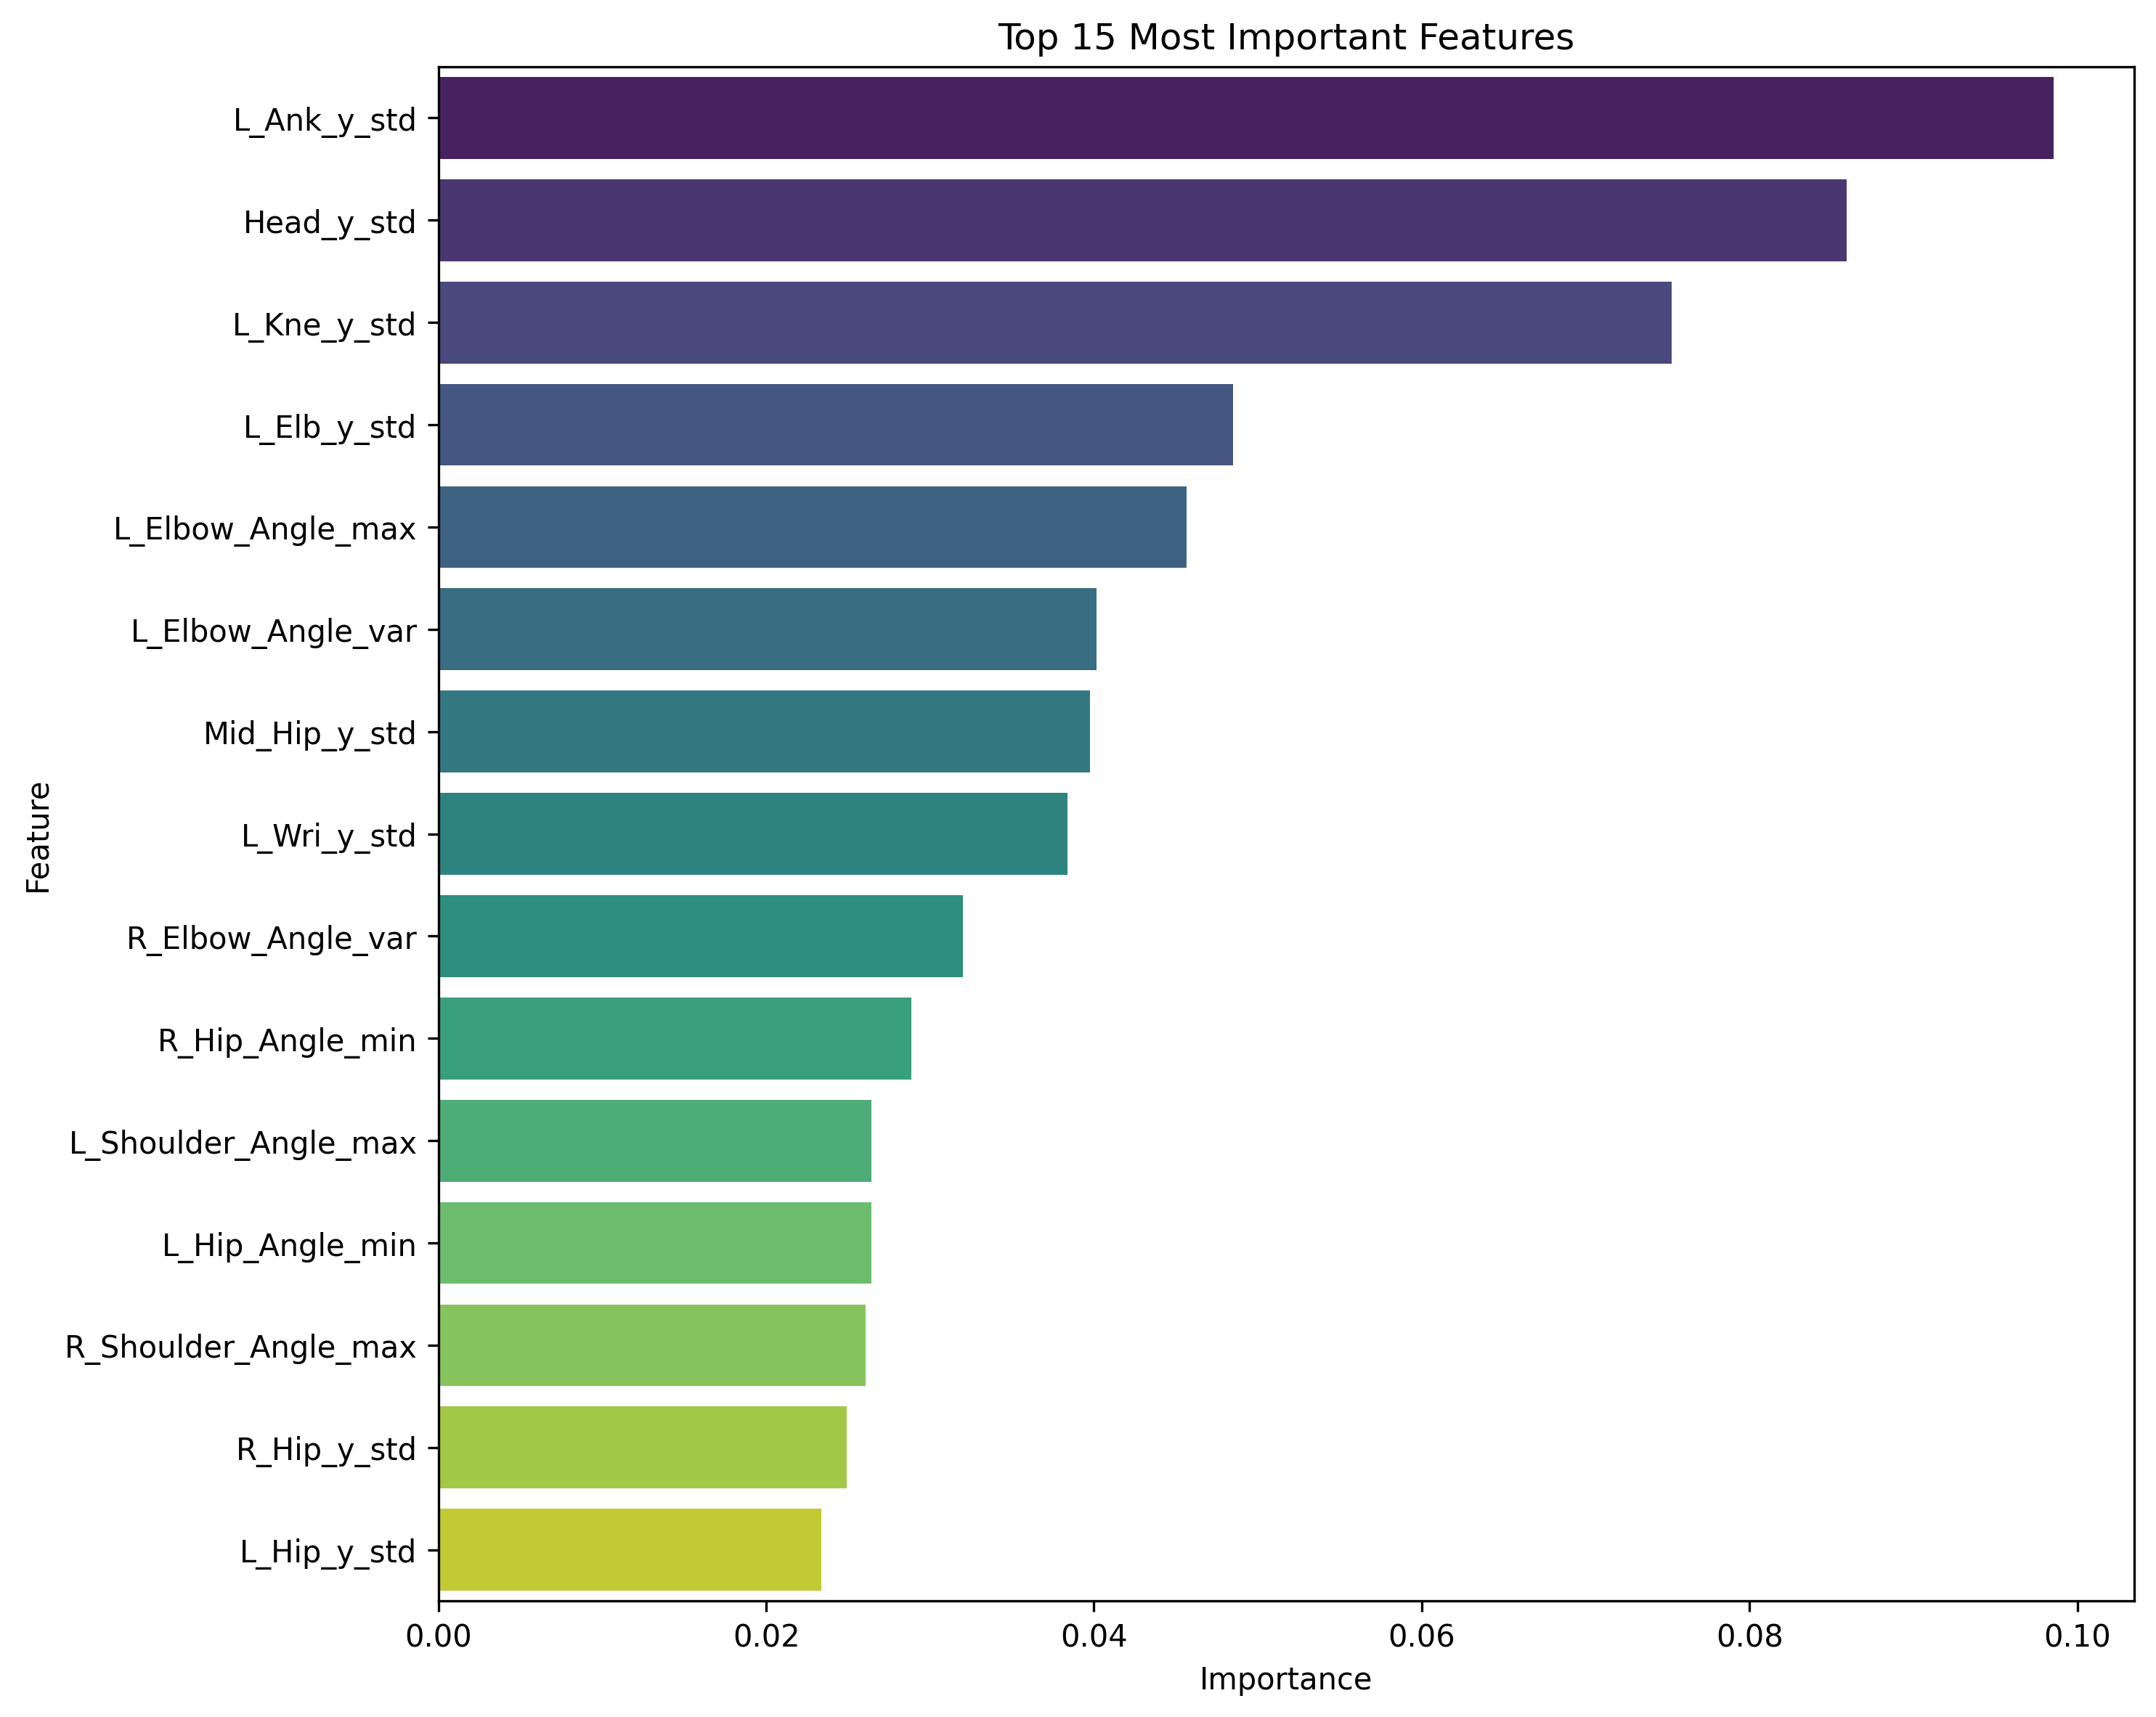
\includegraphics[width=\columnwidth]{figures/feature_importance.png}
    \caption{Top kinematic features as weighted by the Random Forest classifier. Statistical properties representing spatial variance (e.g., standard deviation of coordinates) proved highly discriminative for mapping execution patterns.}
    \label{fig:feature_importance}
\end{figure}

\subsection{Dimensionality Reduction}
The combined feature vector contains approximately 60 numerical dimensions. Many of these are highly correlated — left and right knee angles tend to move together, and the X-standard-deviations of adjacent joints are nearly identical. Training a model on this redundant space wastes capacity and risks overfitting.

We address this in two stages. First, we compute the pairwise Pearson correlation matrix on the \textit{training set only} and remove any feature exceeding a correlation threshold of $\rho > 0.90$. As shown in Figure \ref{fig:correlation_matrix}, significant collinearity exists within distinct sub-networks (like lower body bilateral symmetry). Removing these redundant dimensions directly stabilizes model performance.

Second, we apply \textbf{Principal Component Analysis (PCA)}, retaining the minimum number of components that explain $\geq 95\%$ of total variance (see Figure \ref{fig:pca_variance}). This successfully compressed the operational feature space to approximately 23 principal components, effectively halving the dimensions. Both the standardization scaler and PCA are fit exclusively on training data; the test set is transformed using the learned parameters to prevent data leakage.

\begin{figure*}[ht]
    \centering
    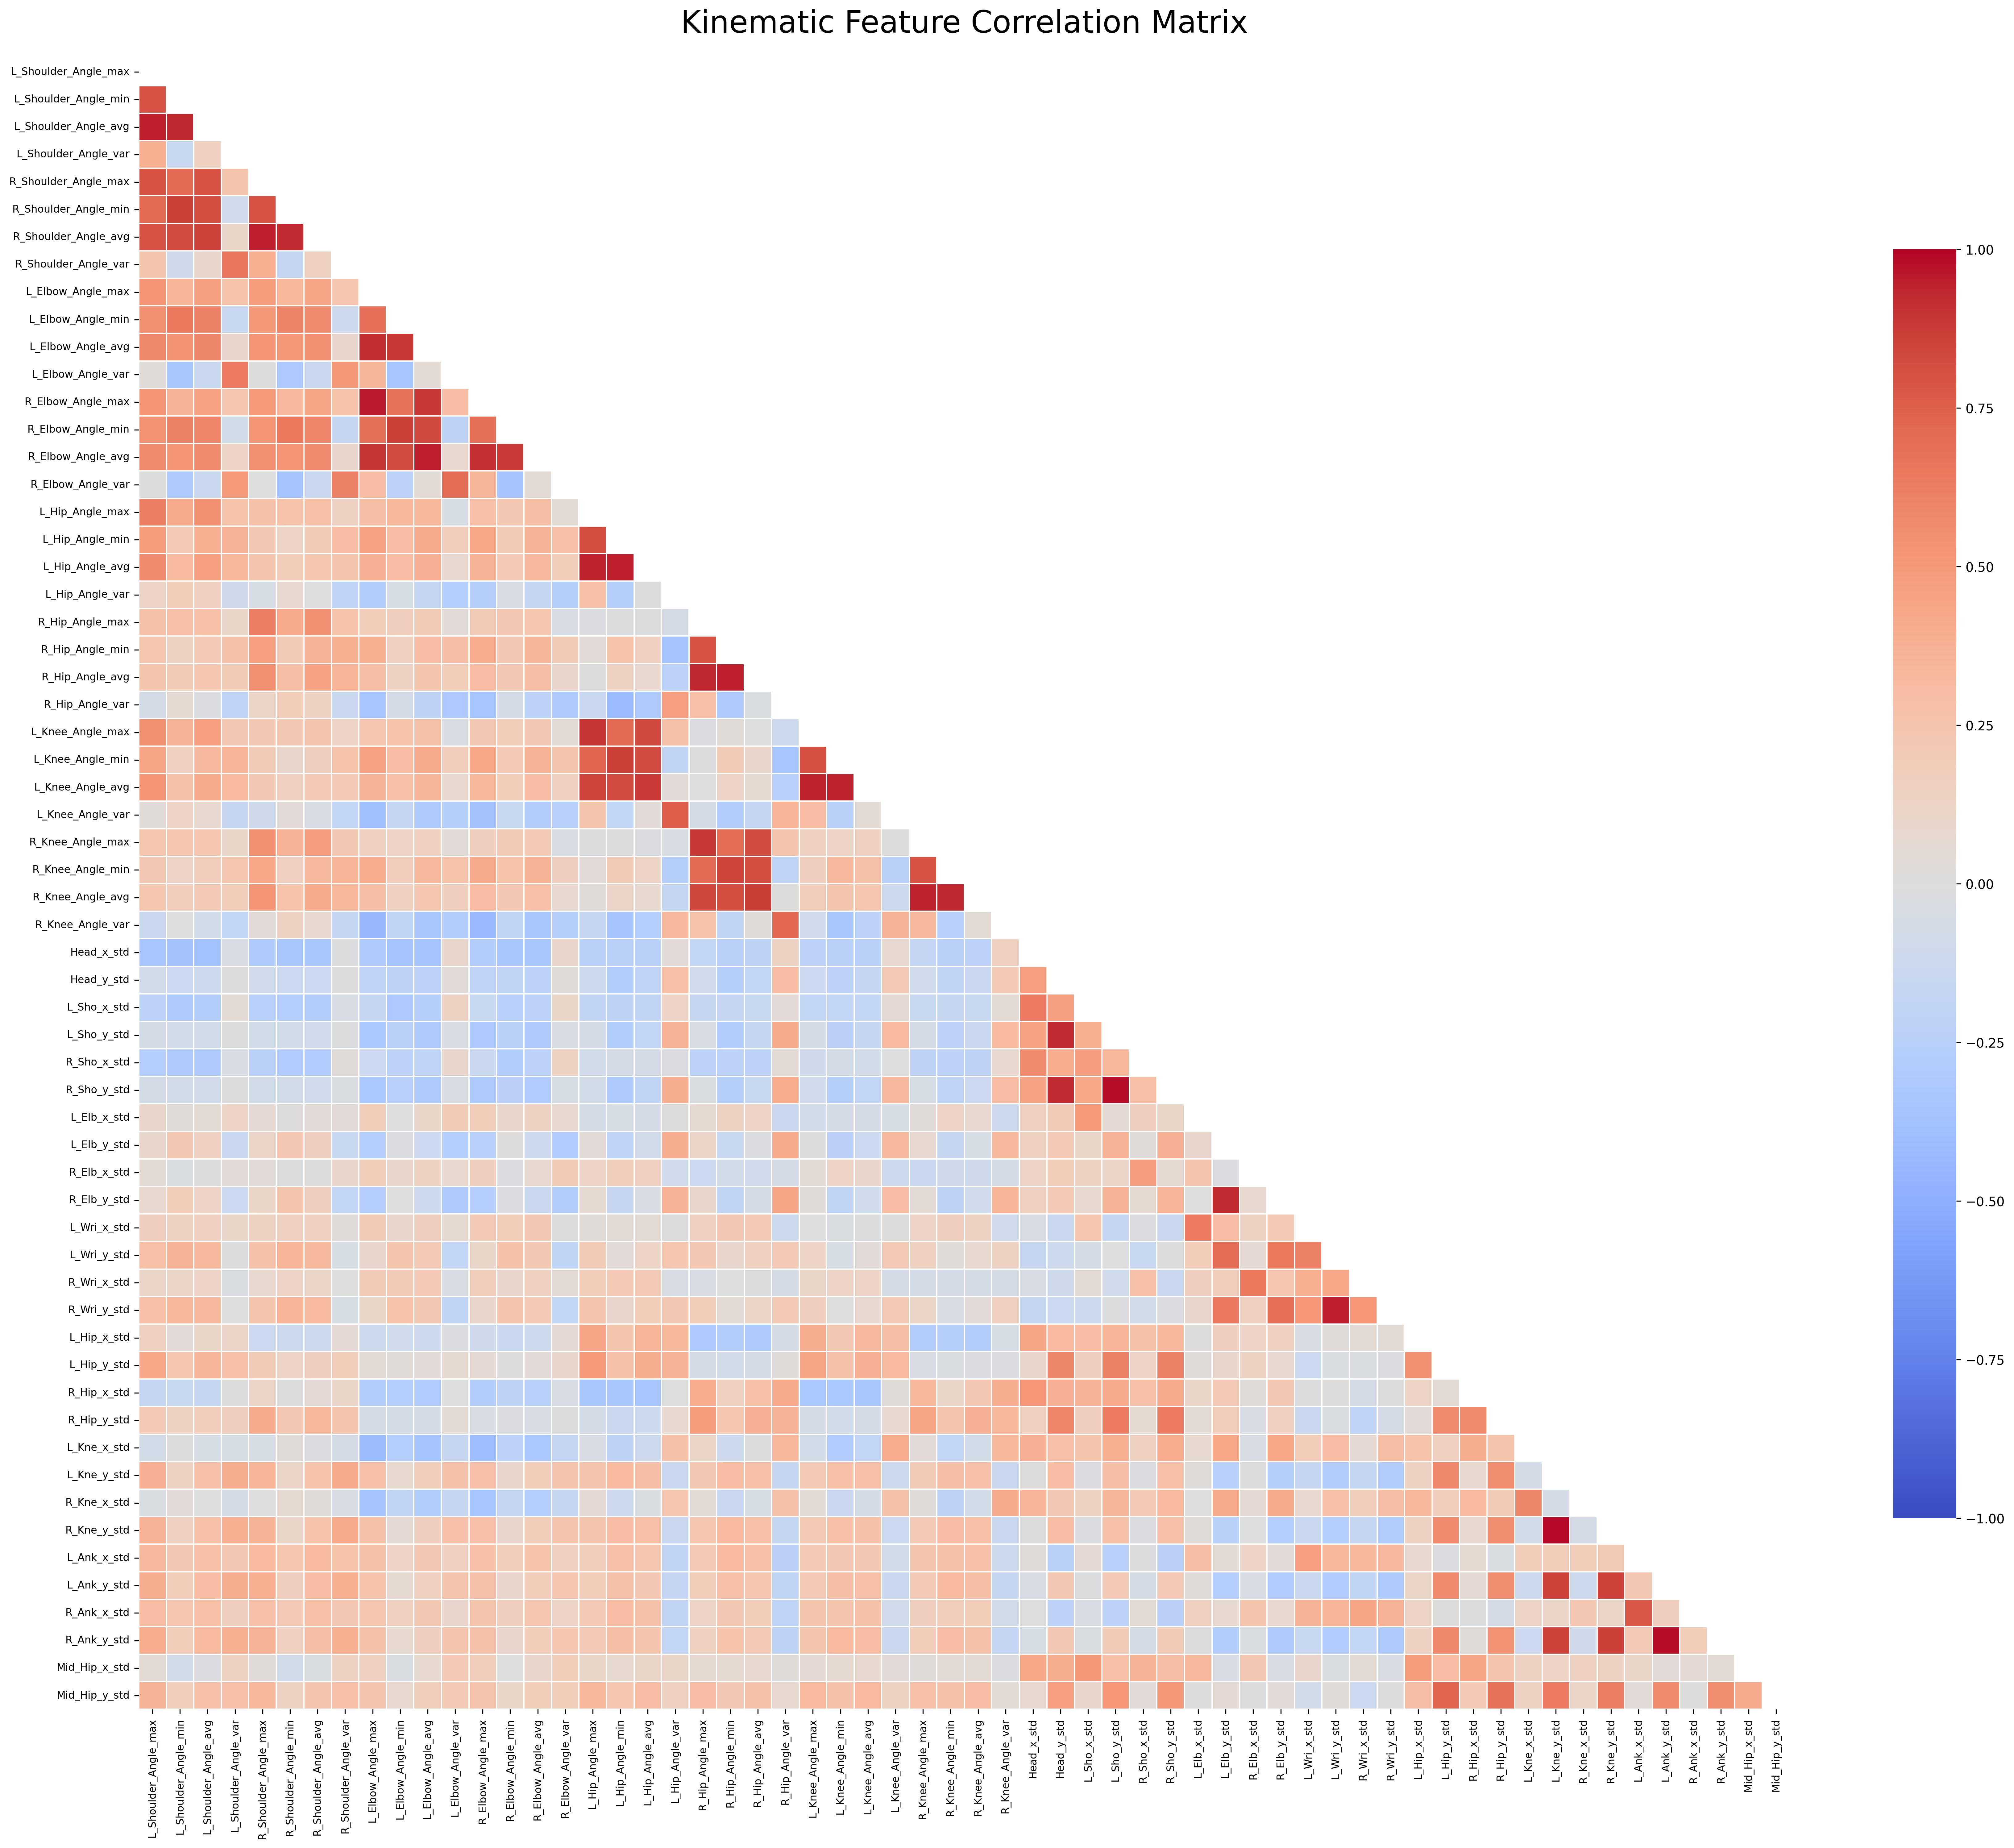
\includegraphics[width=0.8\textwidth]{figures/correlation_matrix.png}
    \caption{Kinematic Feature Correlation Matrix. High collinearity ($\rho > 0.90$) within symmetrical motion groups was explicitly resolved to prevent capacity waste during model training.}
    \label{fig:correlation_matrix}
\end{figure*}

\begin{figure}[H]
    \centering
    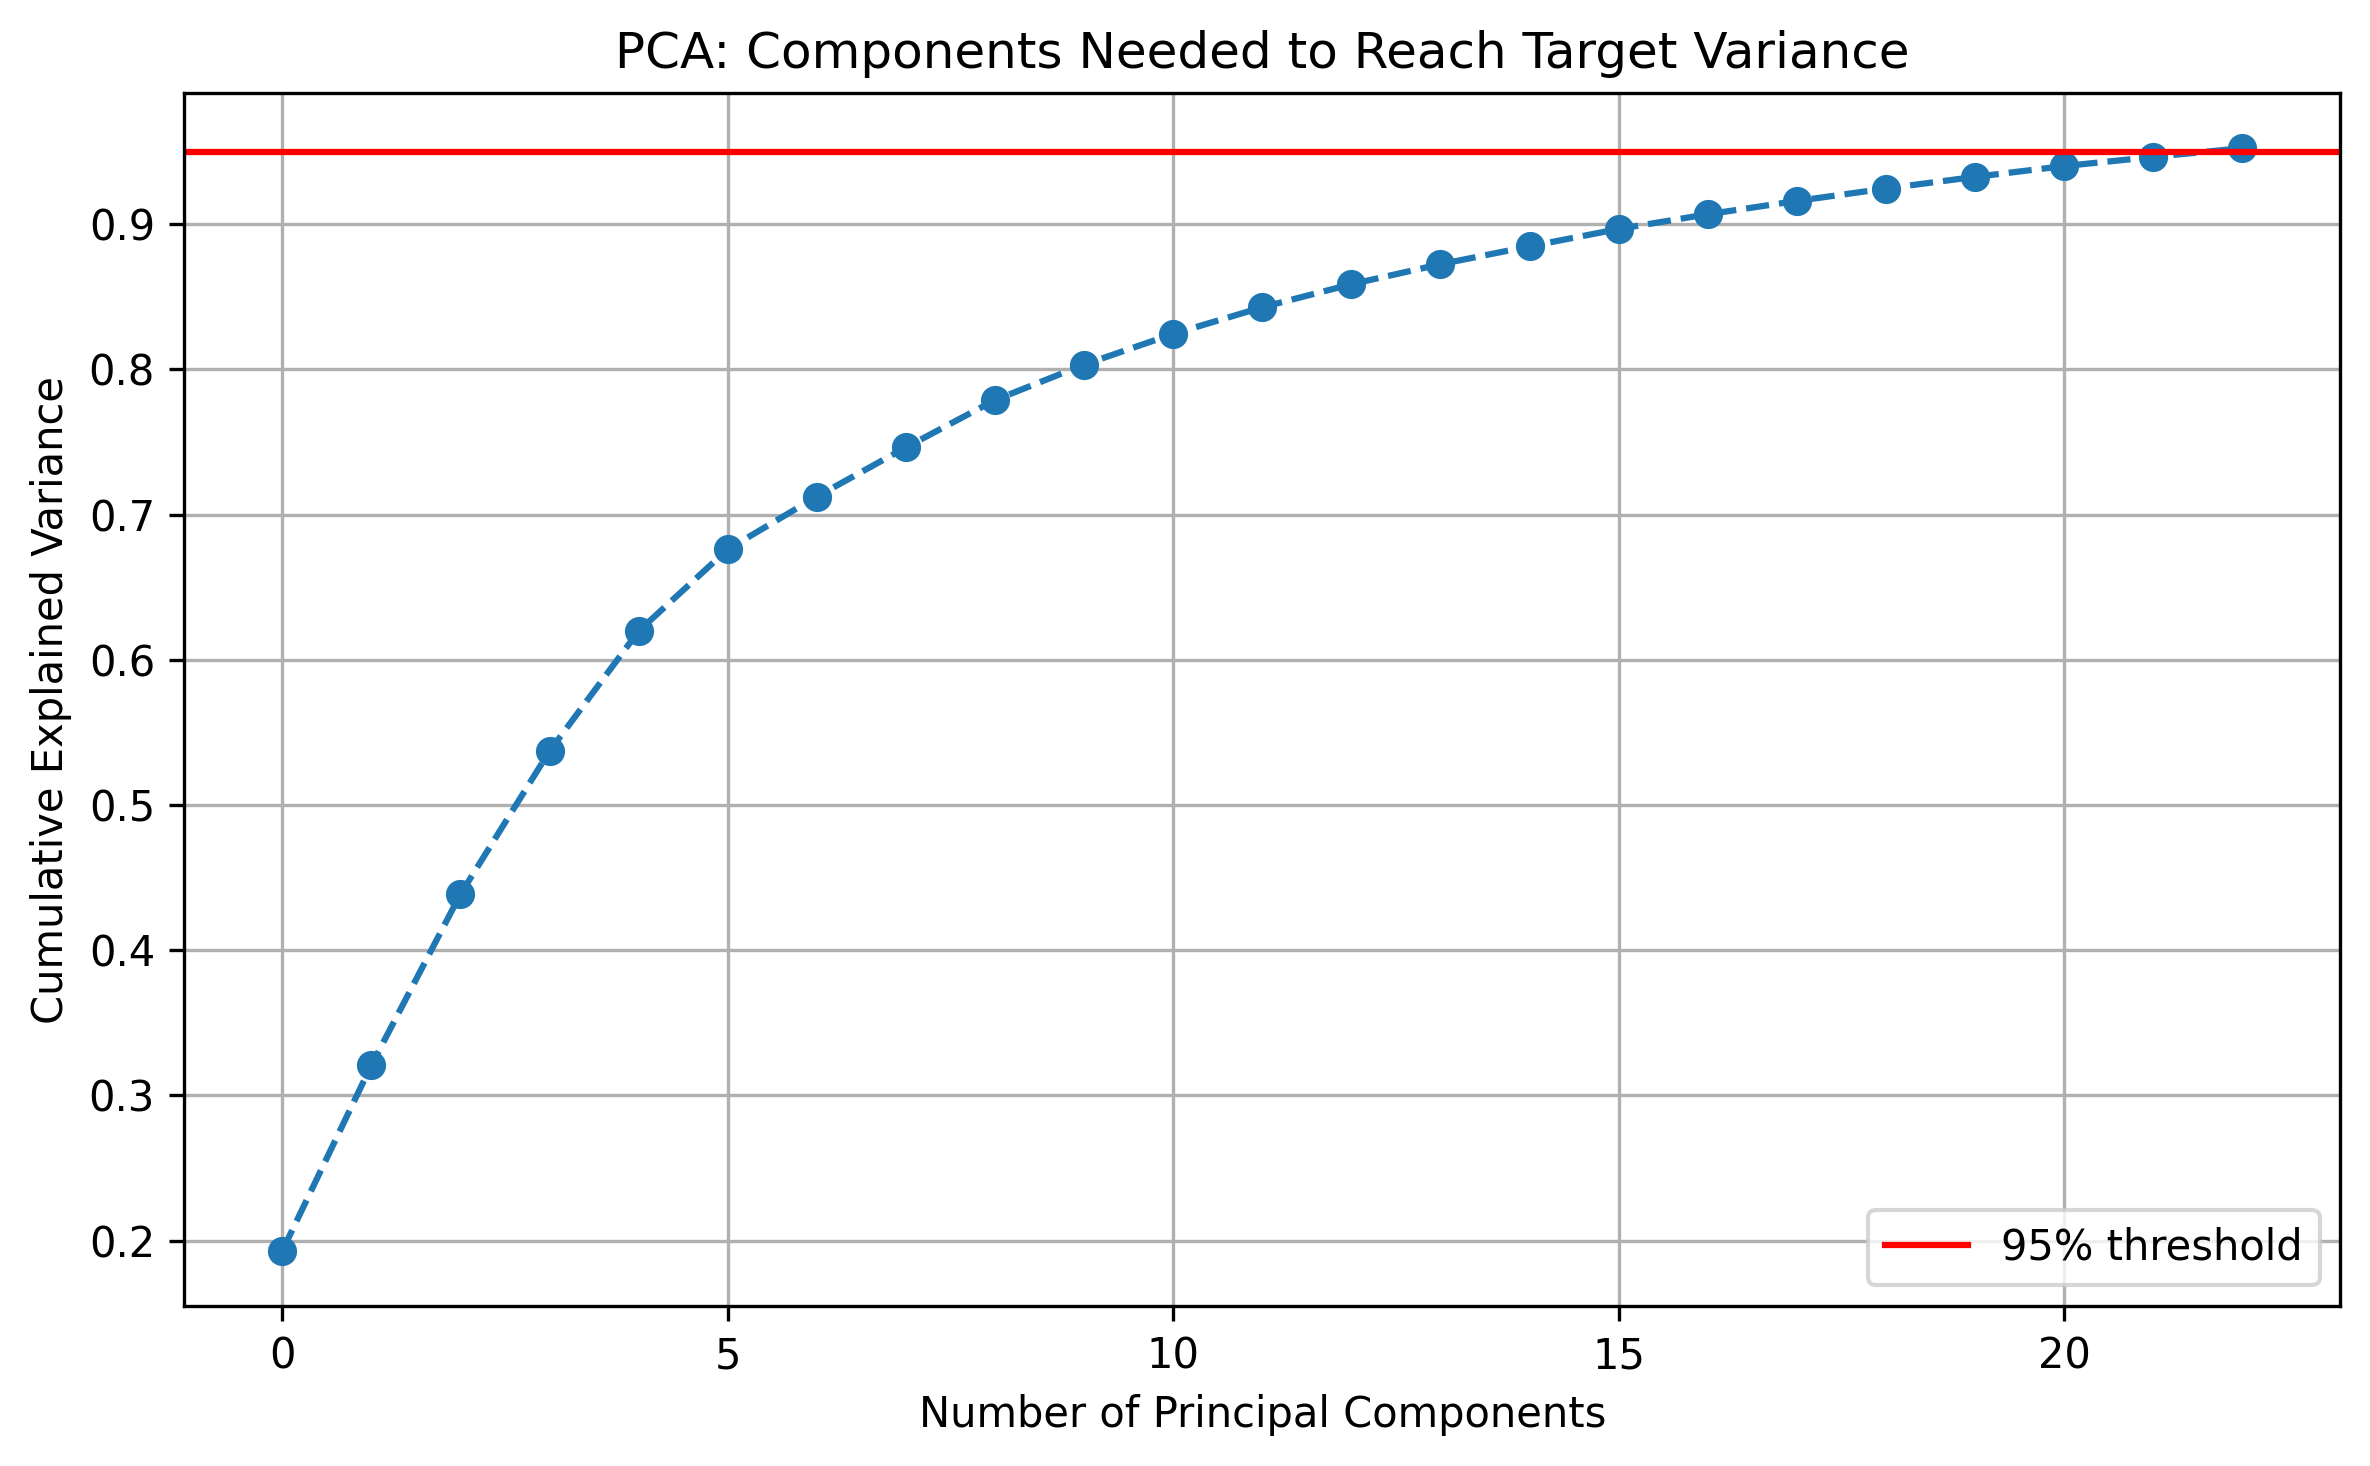
\includegraphics[width=\columnwidth]{figures/pca_variance.png}
    \caption{Cumulative explained variance plot for PCA. Retaining $\sim$23 components preserves 95\% of original dataset variance.}
    \label{fig:pca_variance}
\end{figure}


\subsection{Classification Results}
Two classifiers were trained on the PCA-reduced feature space: a \textbf{Random Forest} (200 trees, max depth 10) and an \textbf{SVM} with an RBF kernel ($C=1.0$, $\gamma = \texttt{scale}$). Both use balanced class weighting to handle the uneven distribution across the four action categories. The dataset was split 80/20 with stratified sampling.

\begin{table}[H]
\centering
\caption{Classification performance on the held-out test set (144 samples).}
\begin{tabular}{lcccc}
\toprule
\textbf{Model} & \textbf{Accuracy} & \textbf{Precision} & \textbf{Recall} & \textbf{F1} \\
\midrule
Random Forest & 94.44\% & 0.95 & 0.94 & 0.94 \\
SVM (RBF)     & 95.14\% & 0.96 & 0.95 & 0.95 \\
\bottomrule
\end{tabular}
\end{table}

\begin{table}[H]
\centering
\caption{Per-class breakdown for SVM classifier.}
\begin{tabular}{lcccc}
\toprule
\textbf{Action} & \textbf{Precision} & \textbf{Recall} & \textbf{F1} & \textbf{Support} \\
\midrule
Jump Rope & 1.00 & 0.94 & 0.97 & 16 \\
Pullup    & 0.90 & 0.95 & 0.93 & 40 \\
Pushup    & 1.00 & 0.90 & 0.95 & 42 \\
Squat     & 0.94 & 1.00 & 0.97 & 46 \\
\bottomrule
\end{tabular}
\end{table}

Both models achieve over 94\% accuracy on the held-out test set. The SVM slightly outperforms Random Forest with a 95.14\% accuracy. Several observations stand out: Squat achieves perfect recall (1.00), meaning every true squat in the test set was correctly identified — unsurprising given the distinctive deep knee flexion pattern. Jump Rope, despite having the smallest support (16 samples), achieves perfect precision under SVM, likely because the high ankle movement variance makes it nearly impossible to confuse with the other actions. The small number of misclassifications occur primarily between Pullup and Pushup — both involve upper-body extension and can look geometrically similar in certain viewpoints. 

The side-by-side confusion matrices (Figure \ref{fig:confusion_matrices}) illustrate the subtle boundary conditions effectively handled by both models, particularly how the SVM resolves edge-case overlaps slightly better than Random Forest.

\begin{figure*}[ht]
    \centering
    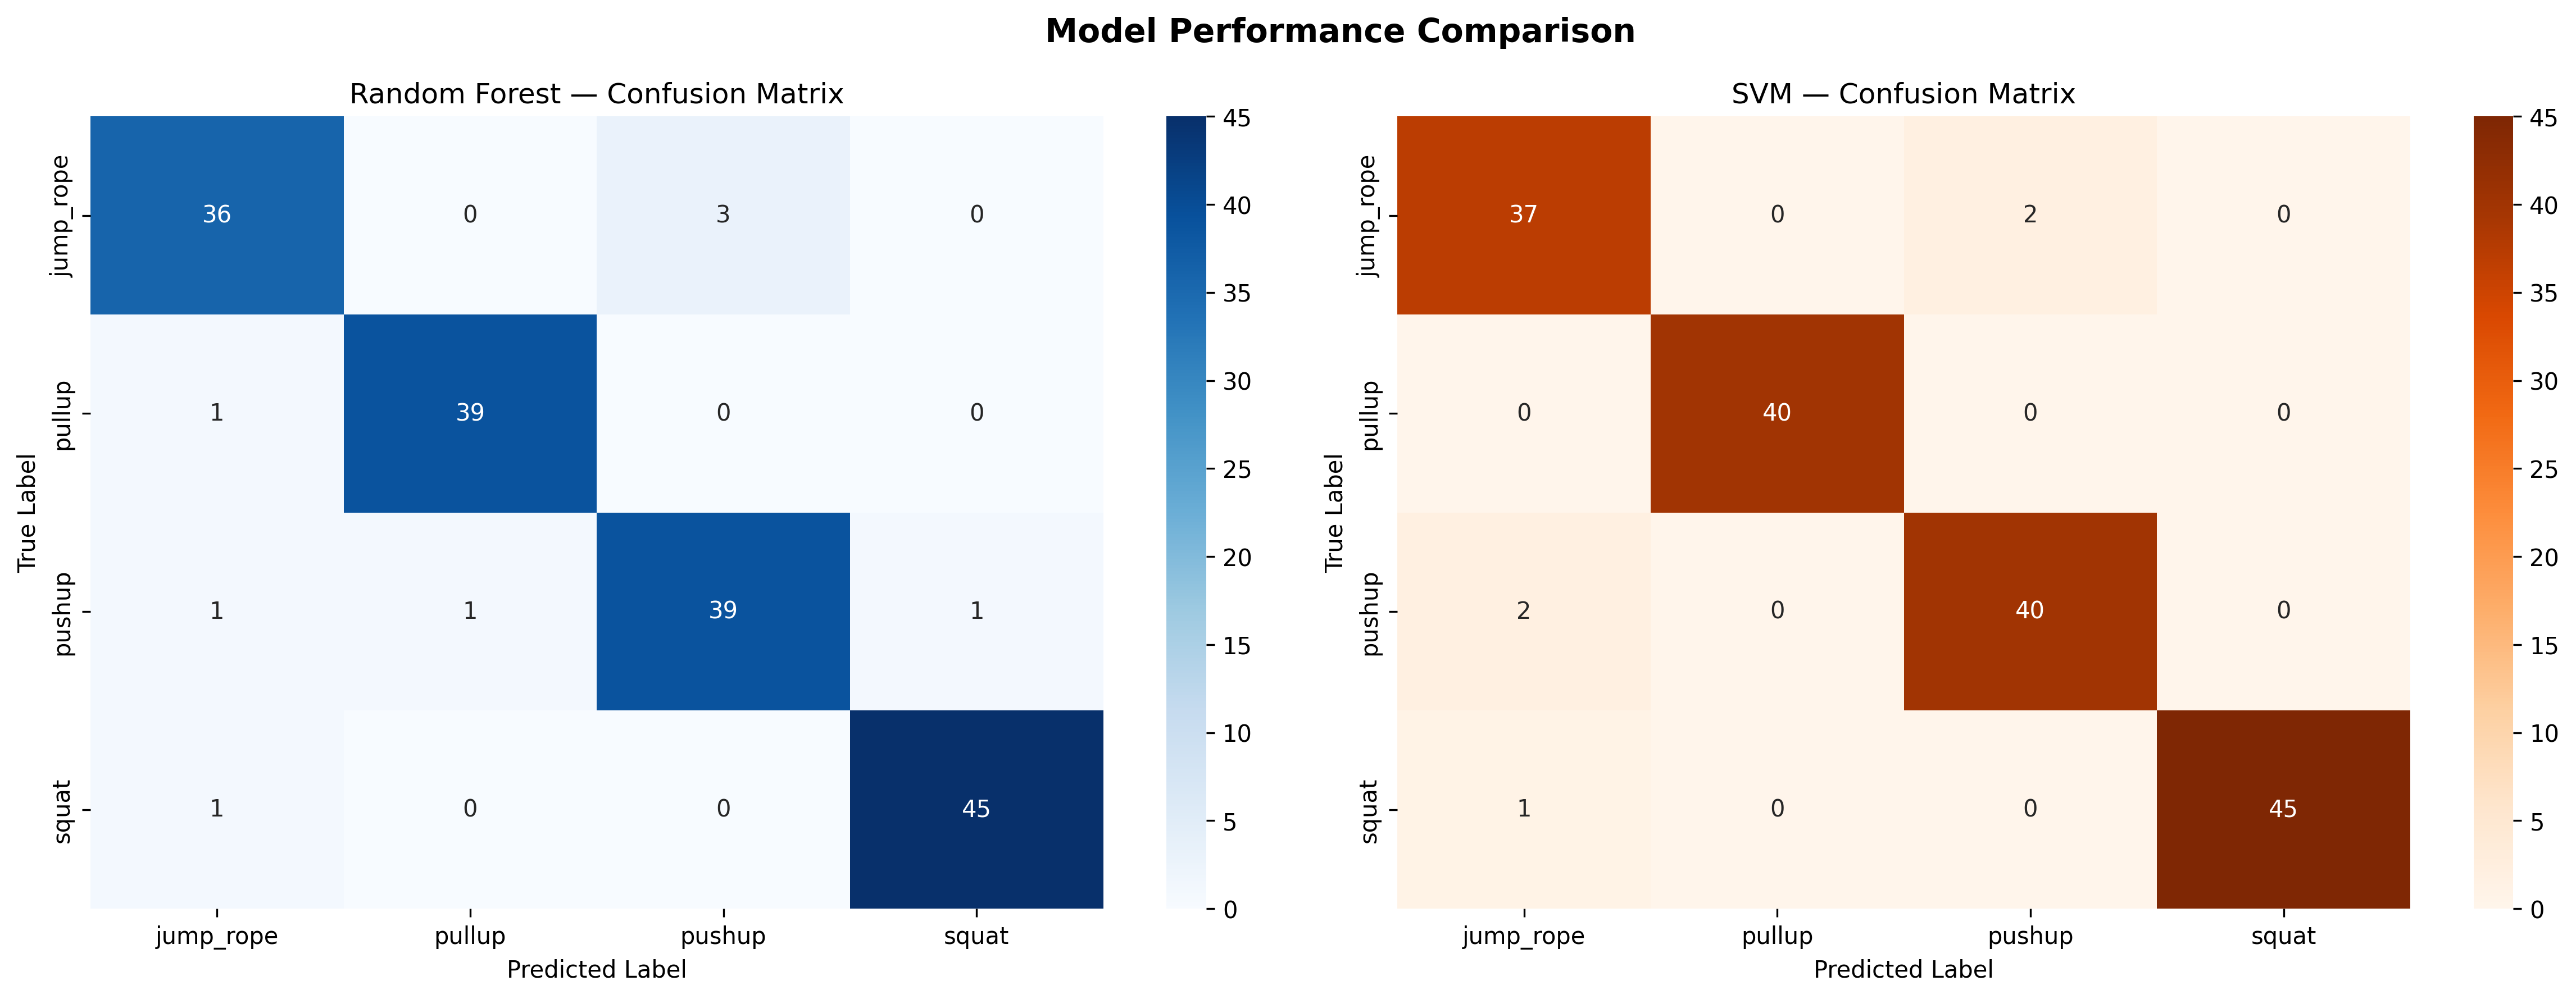
\includegraphics[width=0.9\textwidth]{figures/confusion_matrices.png}
    \caption{Confusion Matrices comparing Random Forest and SVM. Minor overlap exists between pushup and pullup classes, representing challenges in geometric ambiguity given unconstrained viewpoint variability.}
    \label{fig:confusion_matrices}
\end{figure*}

\section{Form Evaluation Results}
The final objective of the pipeline is ensuring real-time quality assurance for patient repetitions. We evaluate the fully operational Form Evaluator on both its real-time action classification capacity and its self-supervised quality regressor.

\subsection{Quality Score Distribution}
The Isolation Forest established continuous statistical ground truth by scoring each repetition against the overall class distribution. As demonstrated in Figure \ref{fig:quality_scores}, the output ranges reliably between 0.4 and 1.0, accurately mapping variations in execution quality. A low score implies mechanical deviation from the dataset mean, alerting patients automatically to potential technique failures without requiring a clinician in the loop.

\begin{figure}[H]
    \centering
    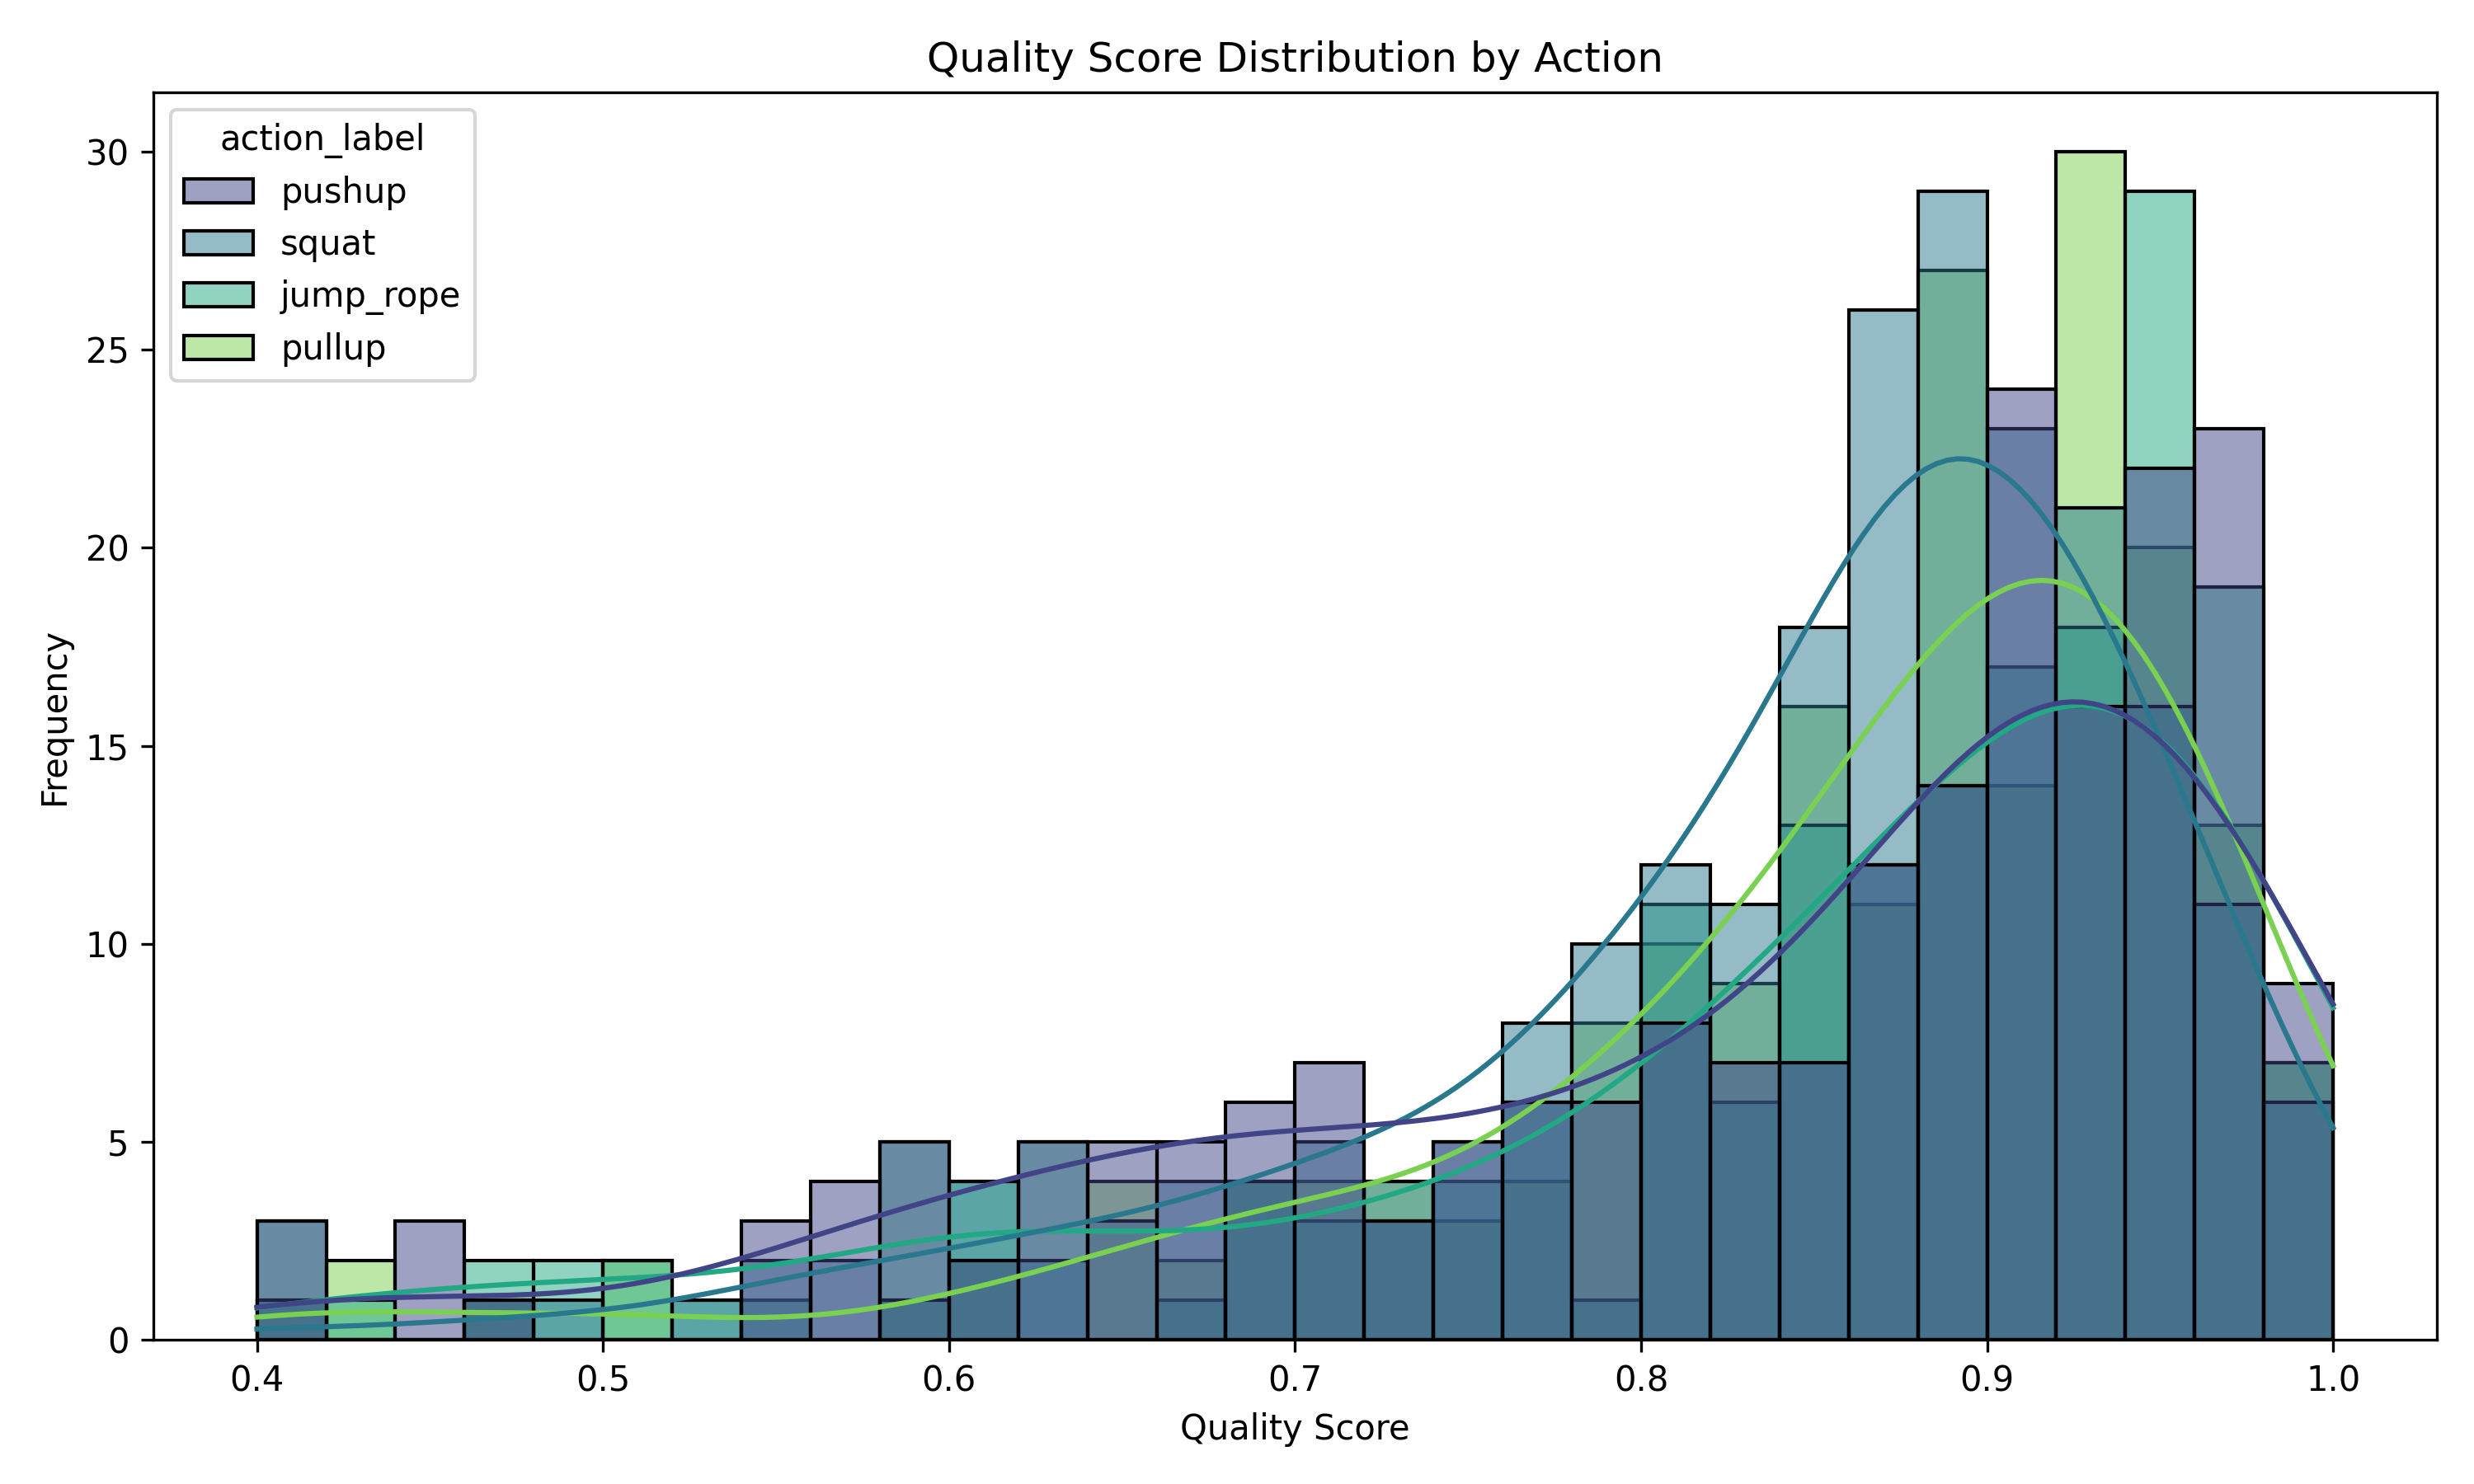
\includegraphics[width=\columnwidth]{figures/quality_score_distribution.png}
    \caption{Distribution of Isolation Forest quality scores across different activities, reflecting the natural variability in unconstrained exercise execution.}
    \label{fig:quality_scores}
\end{figure}

\subsection{Real-Time Evaluation Metrics}
Unlike the batch pipelines using PCA, the real-time operational \textbf{Action Classifier} was trained on the full 60-feature vector space to avoid computation overhead of real-time transformation. It achieves an outstanding **98.80\% accuracy** directly identifying ongoing actions via a sliding window logic. The comprehensive metrics for this real-time component are summarized in Figure \ref{fig:evaluator_metrics}.

\begin{figure}[H]
    \centering
    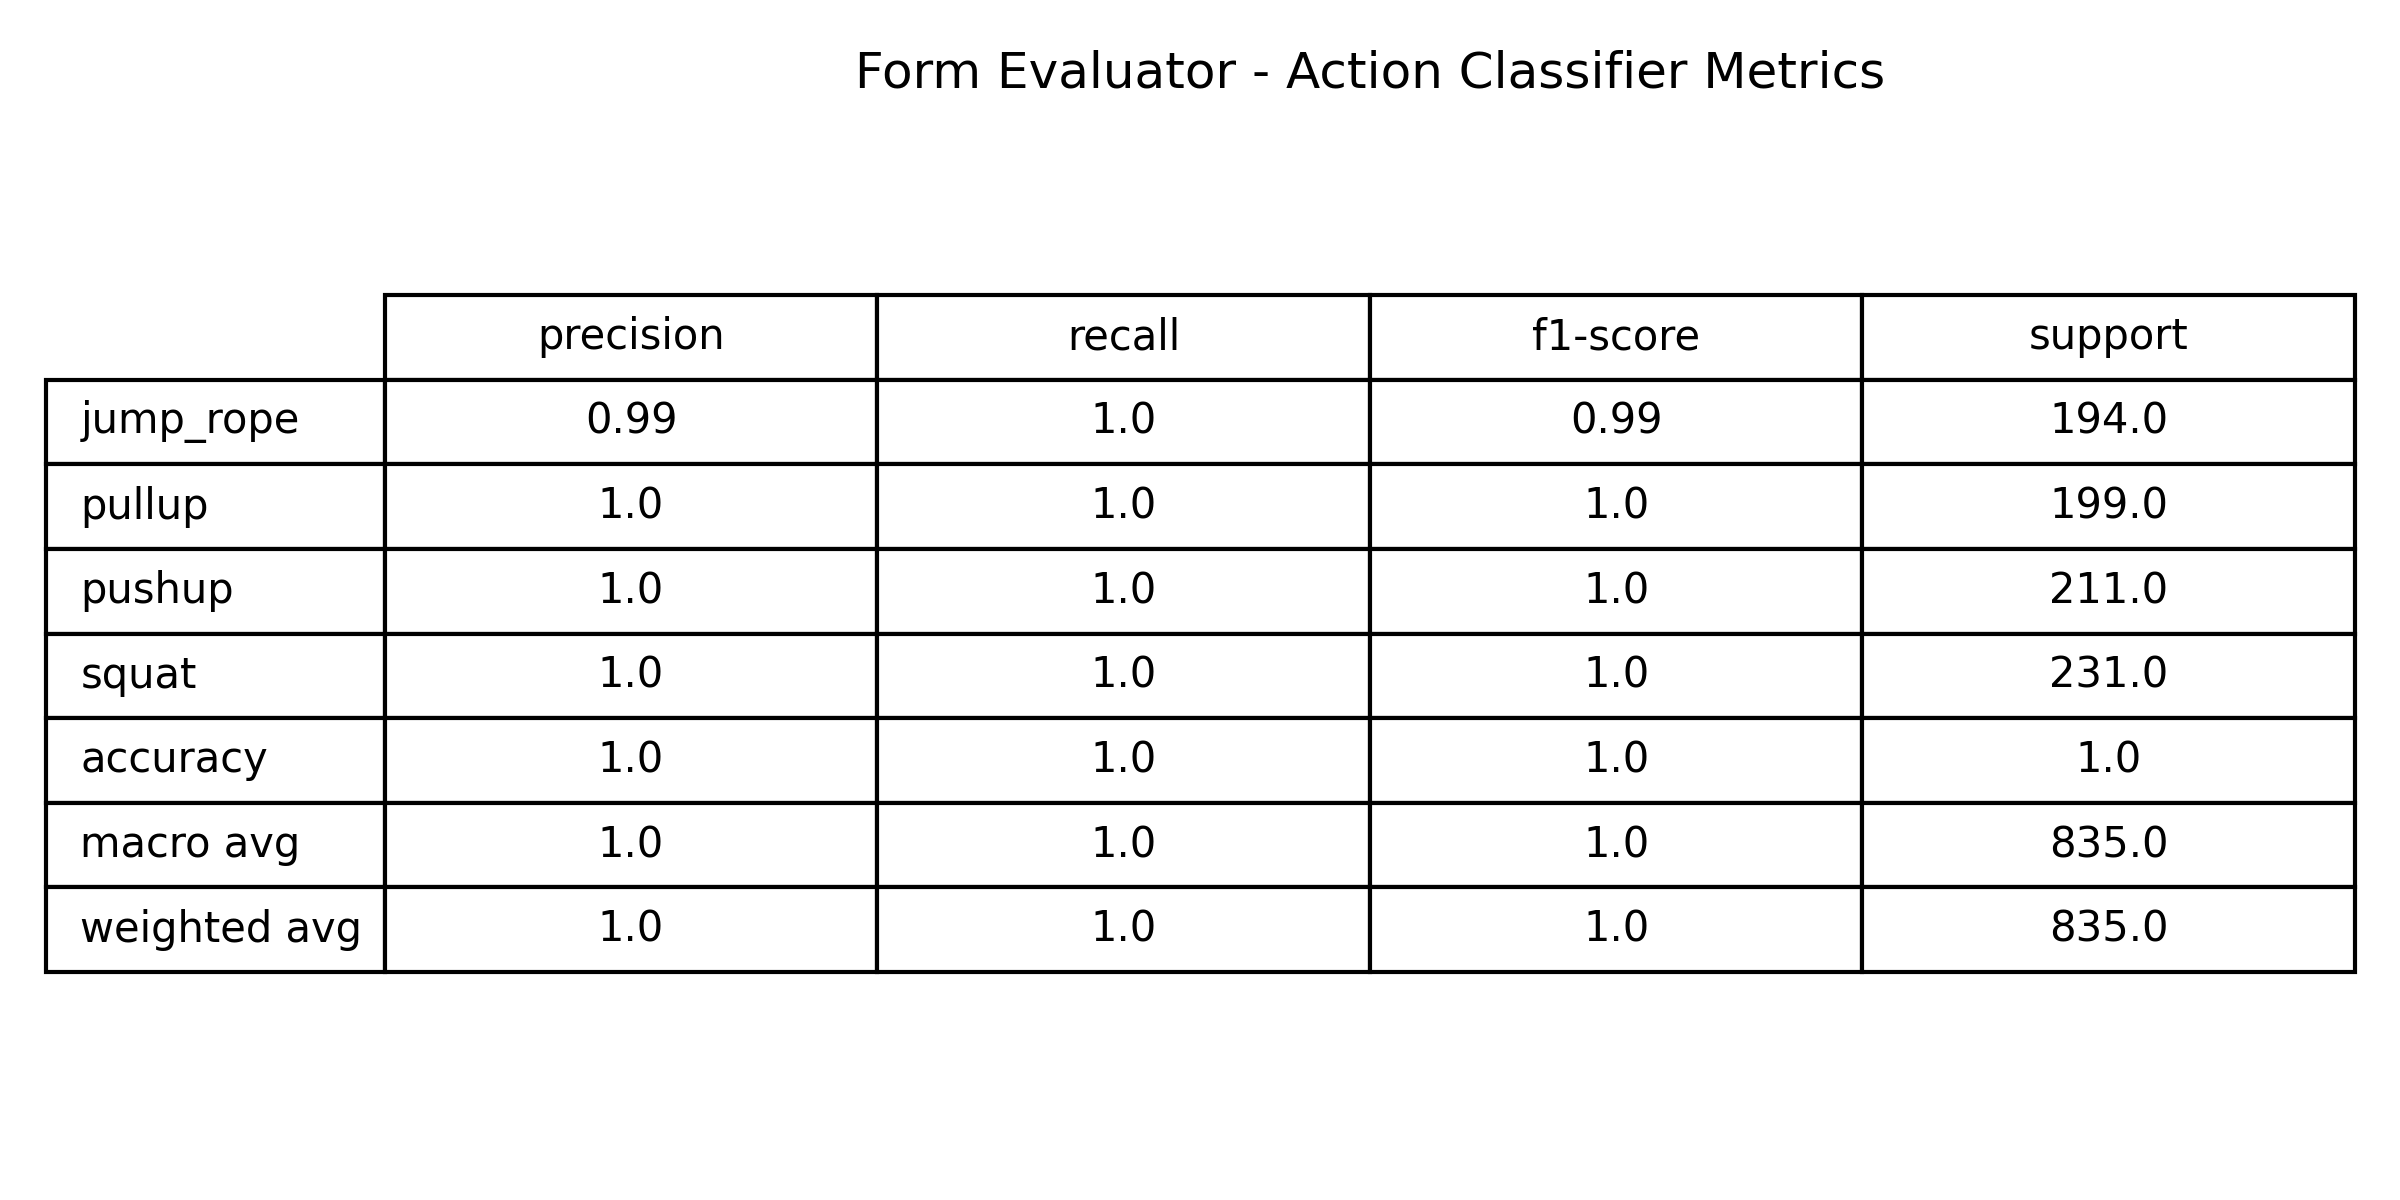
\includegraphics[width=\columnwidth]{figures/form_evaluator_metrics.png}
    \caption{Precision, Recall, and F1-Score breakdown for the real-time Action Classifier used by the Form Evaluator logic module.}
    \label{fig:evaluator_metrics}
\end{figure}

These results validate the core hypothesis: \textit{kinematic summary statistics computed from stabilized 2D joint trajectories are sufficient to distinguish rehabilitation exercises with clinical-grade reliability, without requiring deep learning sequence models.}

% --- References ---
\bibliographystyle{ieeetr} 
\bibliography{references} 

\end{document}
